\begin{frame}{The Coarse-to-Fine Recipe}
  \begin{columns}[T,onlytextwidth]
    \column{0.50\textwidth}
      \begin{itemize}\footnotesize\itemsep0.35em
        \item[\textcolor{red}{$\blacktriangleright$}] Split the $n$ cached keys into $n/b$ contiguous blocks of $b$ tokens. Give each block one cheap summary key: the mean of its keys, a trained landmark token, or a learned compressed token.
        \item[\textcolor{red}{$\blacktriangleright$}] The query $q_t$ scores the summaries, keeps the top-$k$ blocks and runs exact softmax attention over their $kb$ keys. Unlike the fixed patterns, the choice depends on the query.
        \item[\textcolor{red}{$\blacktriangleright$}] Keys read per query: $n/b + kb$ instead of $n$. The sum is smallest at $b = \sqrt{n/k}$, where it equals $2\sqrt{nk}$. Over all $n$ queries: $n^2/b + nkb$ instead of $n^2$.
        \item[\textcolor{red}{$\blacktriangleright$}] Contiguous blocks suit GPUs. A chosen block is one tile of the KV cache, copied from HBM to SRAM in one pass and multiplied on tensor cores like a FlashAttention tile. Scattered single tokens turn every load into a gather.
      \end{itemize}
    \column{0.48\textwidth}
      \centering
      \vspace{0.6em}
      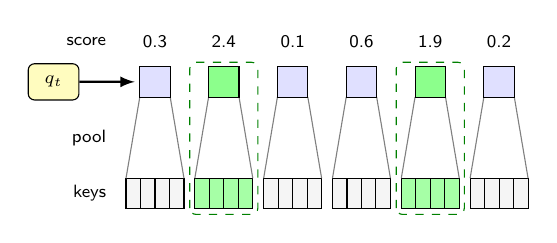
\begin{tikzpicture}[font=\sffamily\scriptsize, >=latex, scale=0.92,
          every node/.style={transform shape},
          tok/.style={draw, minimum width=0.2cm, minimum height=0.42cm, inner sep=0pt},
          summ/.style={draw, minimum width=0.42cm, minimum height=0.42cm, inner sep=0pt},
          qbox/.style={draw, rounded corners=0.08cm, fill=yellow!25, minimum width=0.7cm, minimum height=0.5cm}]
        % six blocks of b = 4 keys; block i spans x = 0.95i to 0.95i + 0.8
        \foreach \i/\s/\sel in {0/0.3/0, 1/2.4/1, 2/0.1/0, 3/0.6/0, 4/1.9/1, 5/0.2/0} {
          \pgfmathsetmacro{\xl}{0.95*\i}
          \pgfmathsetmacro{\xc}{0.95*\i+0.4}
          \ifnum\sel=1
            \def\tf{green!35}\def\sf{green!45}
            \draw[green!50!black, dashed, rounded corners=0.08cm] (\xl-0.07, -0.08) rectangle (\xl+0.87, 2.02);
          \else
            \def\tf{gray!8}\def\sf{blue!12}
          \fi
          \foreach \j in {0,...,3}
            \node[tok, fill=\tf] at (\xl+0.1+0.2*\j, 0.21) {};
          \draw[gray] (\xl, 0.42) -- (\xc-0.21, 1.54);
          \draw[gray] (\xl+0.8, 0.42) -- (\xc+0.21, 1.54);
          \node[summ, fill=\sf] at (\xc, 1.75) {};
          \node at (\xc, 2.3) {\s};
        }
        \node[qbox] (q) at (-1.0, 1.75) {$q_t$};
        \draw[->, thick] (q.east) -- (0.12, 1.75);
        \node[anchor=east] at (-0.15, 2.3) {score};
        \node[anchor=east] at (-0.15, 0.98) {pool};
        \node[anchor=east] at (-0.15, 0.21) {keys};
      \end{tikzpicture}\\[0.4em]
      {\scriptsize $n = 24$ keys, $b = 4$, $k = 2$: the query scores 6 summaries and reads the 8 keys of the green blocks exactly, 14 reads instead of 24.\par}
      \vspace{0.6em}
      \begin{itemize}\footnotesize
        \item[\textcolor{red}{$\blacktriangleright$}] \textbf{Worked number:} $n = 65{,}536$ and $k = 16$ give $b = 64$, so 1,024 summaries plus 1,024 exact keys: 2,048 reads instead of 65,536, a 32$\times$ cut.
      \end{itemize}
  \end{columns}
\end{frame}

\begin{frame}{Landmark Tokens Gate Whole Blocks}
  \begin{columns}[T,onlytextwidth]
    \column{0.50\textwidth}
      \begin{itemize}\footnotesize\itemsep0.3em
        \item[\textcolor{red}{$\blacktriangleright$}] Mohtashami and Jaggi (EPFL) append a \textbf{landmark token} to every block of $b$ tokens. Training makes its key the summary of the block, so attention itself does the retrieval.
        \item[\textcolor{red}{$\blacktriangleright$}] \textbf{Grouped softmax.} Query token $i$ takes one softmax over its own block and all other landmarks, and a separate softmax inside each other block. A token $j$ in another block gets the weight
          \[ a_{ij} = P_{ij}\, P_{i,p_j}, \]
          its probability inside its block times that of its block's landmark $p_j$, so the landmark gates the whole block.
        \item[\textcolor{red}{$\blacktriangleright$}] \textbf{Inference.} Each token and head loads the top-$k$ blocks by landmark score; only the landmarks must stay on the GPU. Blocks of 50 tokens cut attention work about 50-fold.
        \item[\textcolor{red}{$\blacktriangleright$}] \textbf{LLaMA 7B}, fine-tuned for 15,000 steps at context length 512, finds a hidden pass key in 98\% of 50 prompts at 32,070 tokens. The base model fails just past its 2,048-token training length.
      \end{itemize}
    \column{0.48\textwidth}
      \centering
      \vspace{0.4em}
      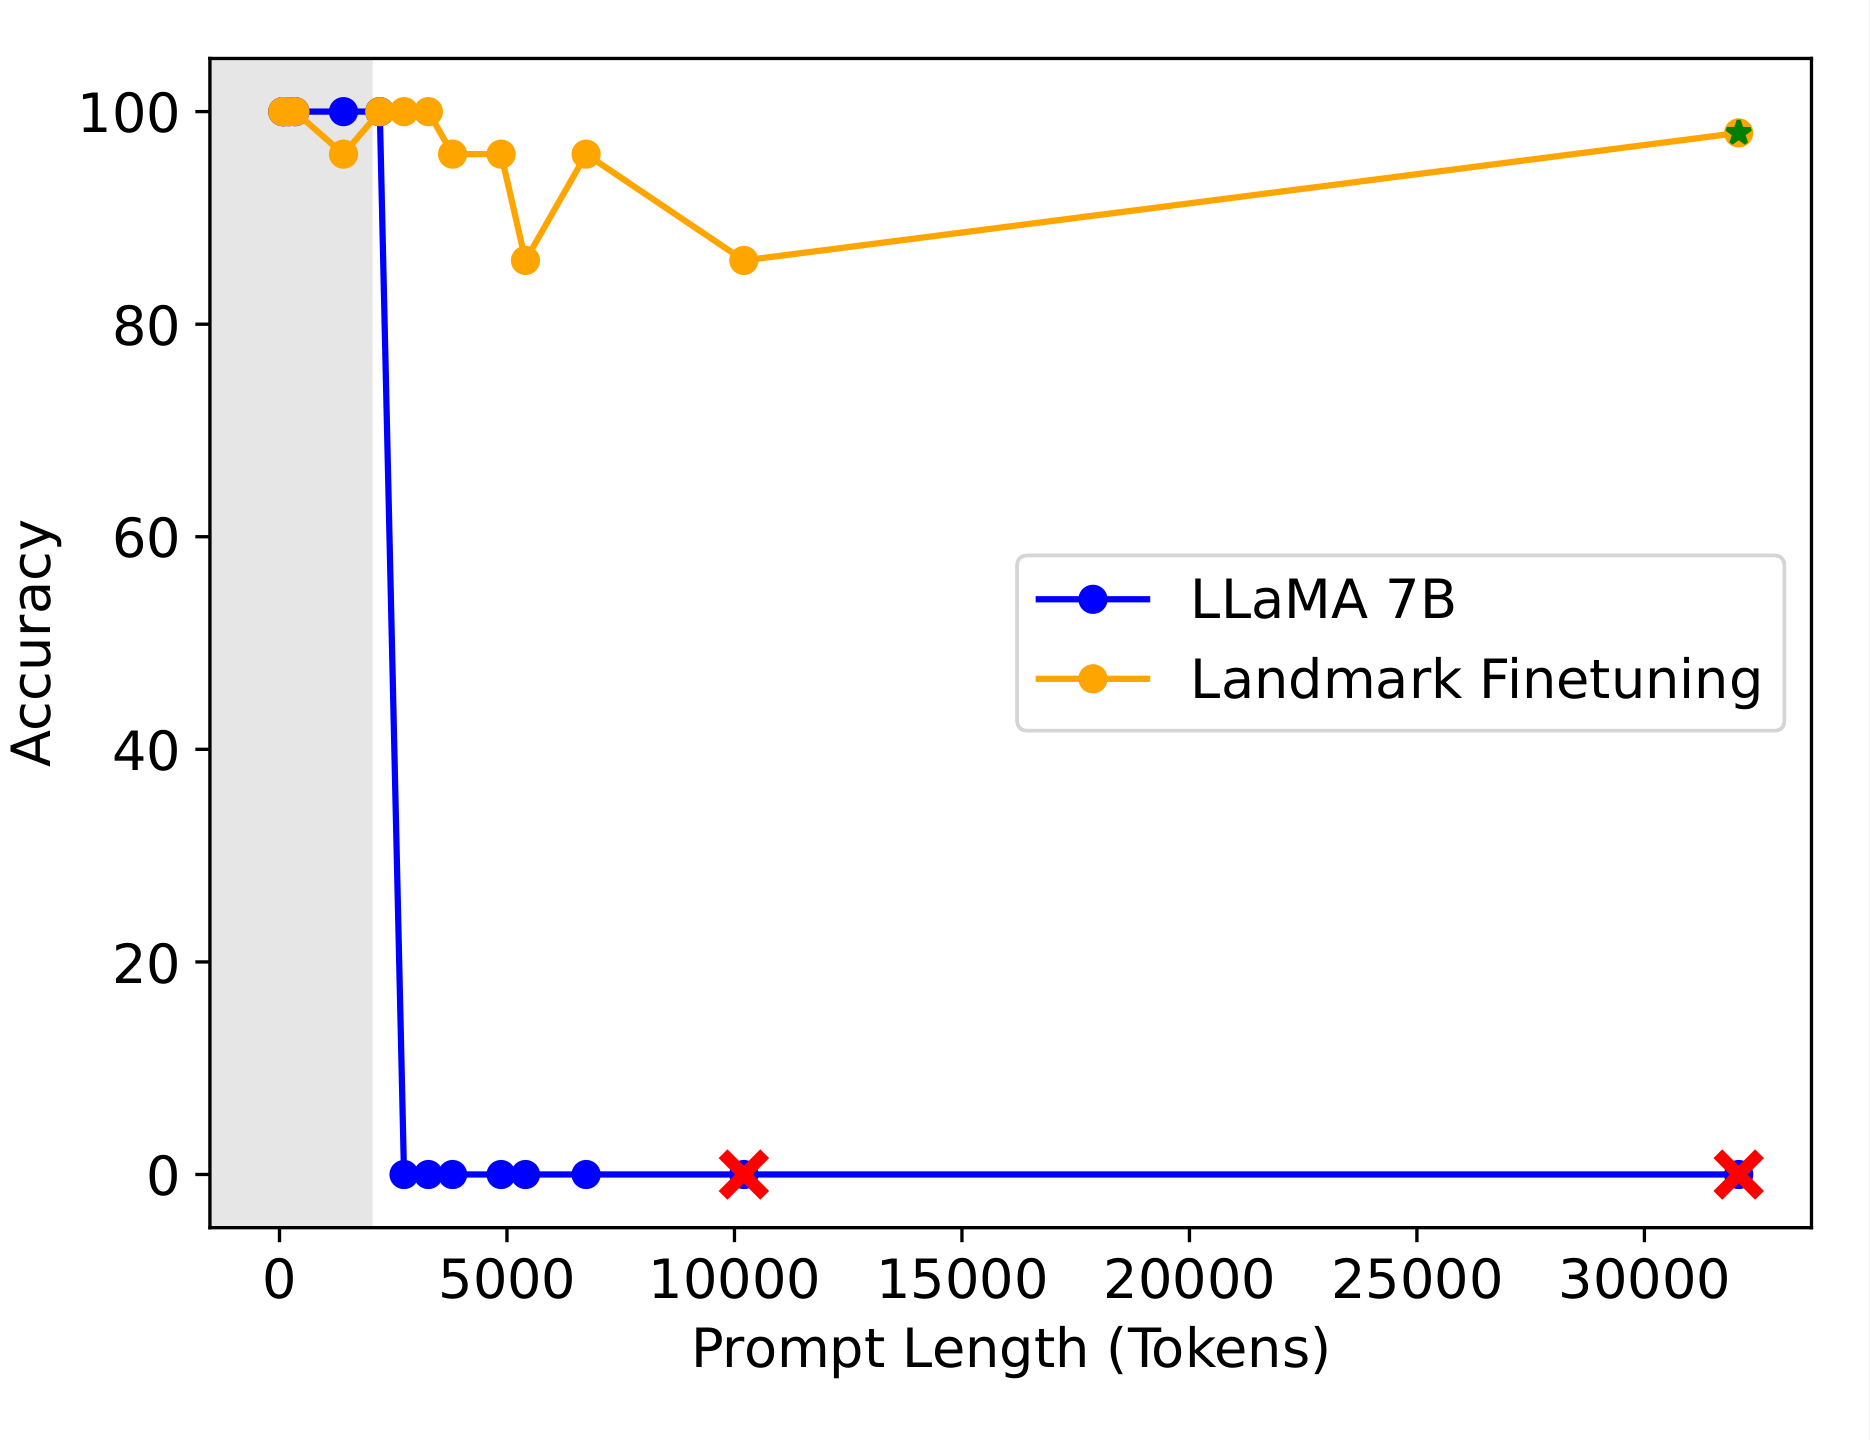
\includegraphics[width=\linewidth,height=0.50\textheight,keepaspectratio]{images/long-context/landmark_fig3b_passkey_retrieval.png}\\[0.2em]
      {\scriptsize Pass-key accuracy against prompt length; grey band: LLaMA's training lengths, red crosses: out of memory, green star: cache offloaded to CPU, 5 blocks per head. Mohtashami \& Jaggi, ``Random-Access Infinite Context Length for Transformers,'' NeurIPS 2023, \href{https://arxiv.org/abs/2305.16300v2}{arXiv:2305.16300v2}, Figure~3(b).\par}
  \end{columns}
\end{frame}

\begin{frame}{MoBA: Routing Queries to Key Blocks}
  \begin{columns}[T,onlytextwidth]
    \column{0.50\textwidth}
      \begin{itemize}\footnotesize\itemsep0.3em
        \item[\textcolor{red}{$\blacktriangleright$}] Lu et al.\ (Moonshot AI) apply mixture-of-experts (MoE) top-$k$ gating to attention: blocks of keys and values are the experts.
        \item[\textcolor{red}{$\blacktriangleright$}] The gate has no parameters. Query $t$ scores block $i$ by
          \[ r_i = \big\langle q_t,\ \operatorname{mean}(K_{[i]}) \big\rangle \]
          ($K_{[i]}$: the $b$ keys of block $i$) and attends to the $k$ highest-scoring blocks.
        \item[\textcolor{red}{$\blacktriangleright$}] Future blocks are excluded; the query's own block is always one of the $k$, with a causal mask, like a shared expert.
        \item[\textcolor{red}{$\blacktriangleright$}] Queries are regrouped by block for variable-length FlashAttention (panel b) and merged by online softmax.
      \end{itemize}
    \column{0.48\textwidth}
      \centering
      \vspace{0.3em}
      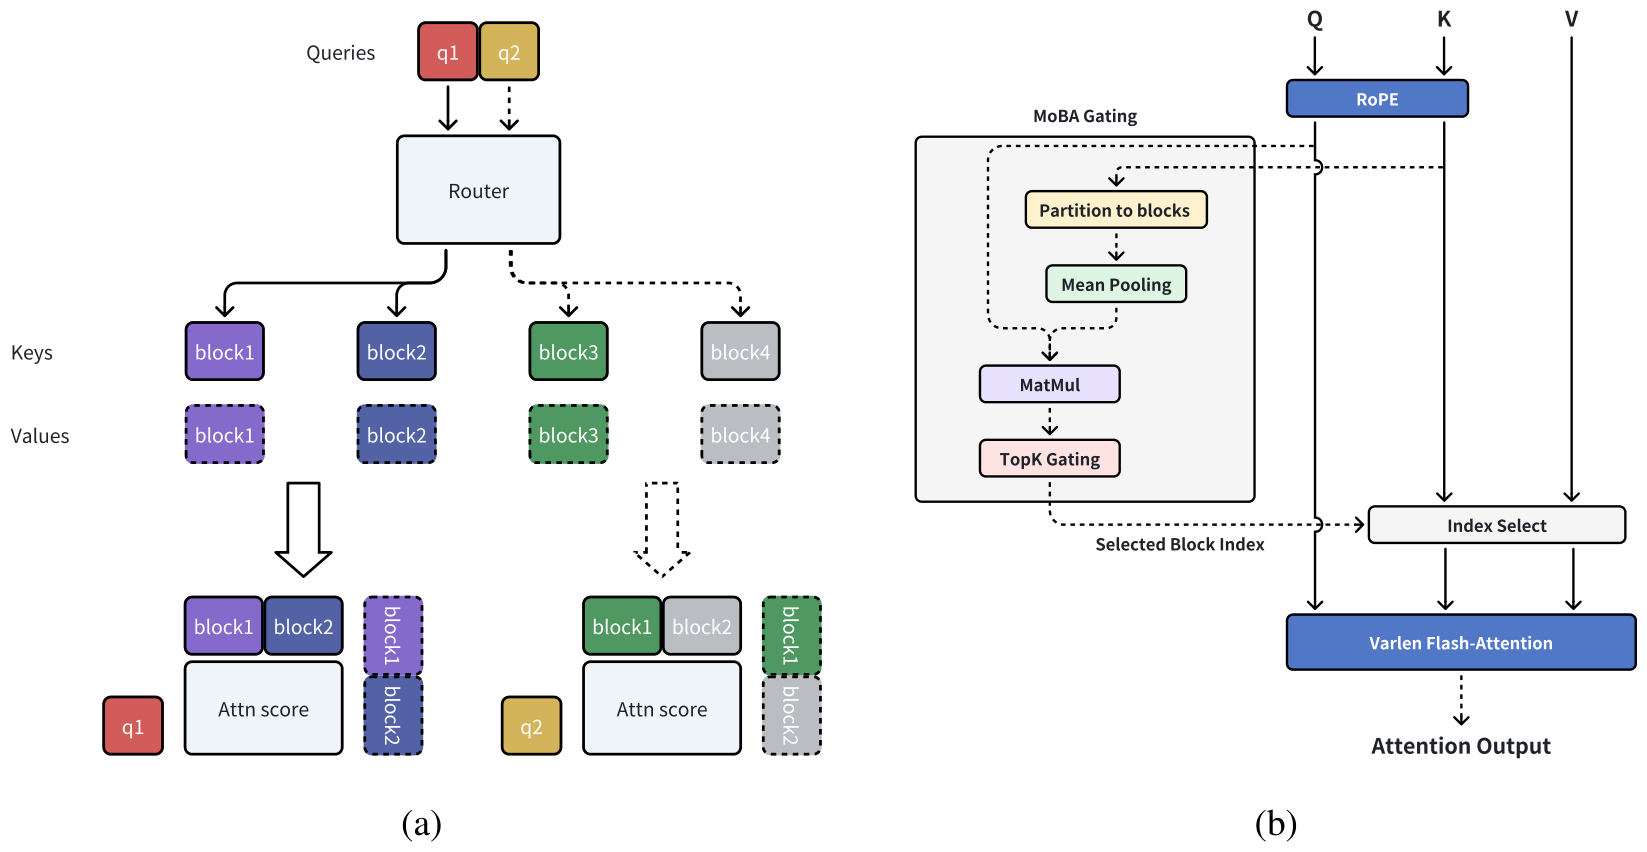
\includegraphics[width=\linewidth,height=0.44\textheight,keepaspectratio]{images/long-context/moba_fig1_running_example_and_kernel.png}\\[0.2em]
      {\scriptsize (a) Two queries, four blocks, top-2 routing; (b) the gate in front of variable-length FlashAttention. Lu et al., ``MoBA: Mixture of Block Attention for Long-Context LLMs,'' 2025, \href{https://arxiv.org/abs/2502.13189v1}{arXiv:2502.13189v1}, Figure~1.\par}
  \end{columns}
  \vspace{0.3em}
  \begin{itemize}\footnotesize\itemsep0.15em
    \item[\textcolor{red}{$\blacktriangleright$}] \textbf{Same parameters as full attention}, so layers can switch. A 1M-token Llama 3.1 8B trained 100B more tokens with MoBA ($b = 4096$, $k = 12$, last 3 of 32 layers dense; MoBA in prefill only) scores 0.7818 on RULER at 128K, full attention 0.7849.
    \item[\textcolor{red}{$\blacktriangleright$}] Attention runs 6.5$\times$ faster than FlashAttention on a 1M-token prefill and 16$\times$ at 10M. MoBA serves long-context requests in Moonshot's Kimi assistant.
  \end{itemize}
\end{frame}

\begin{frame}{NSA: Three Branches and a Gate}
  \centering
  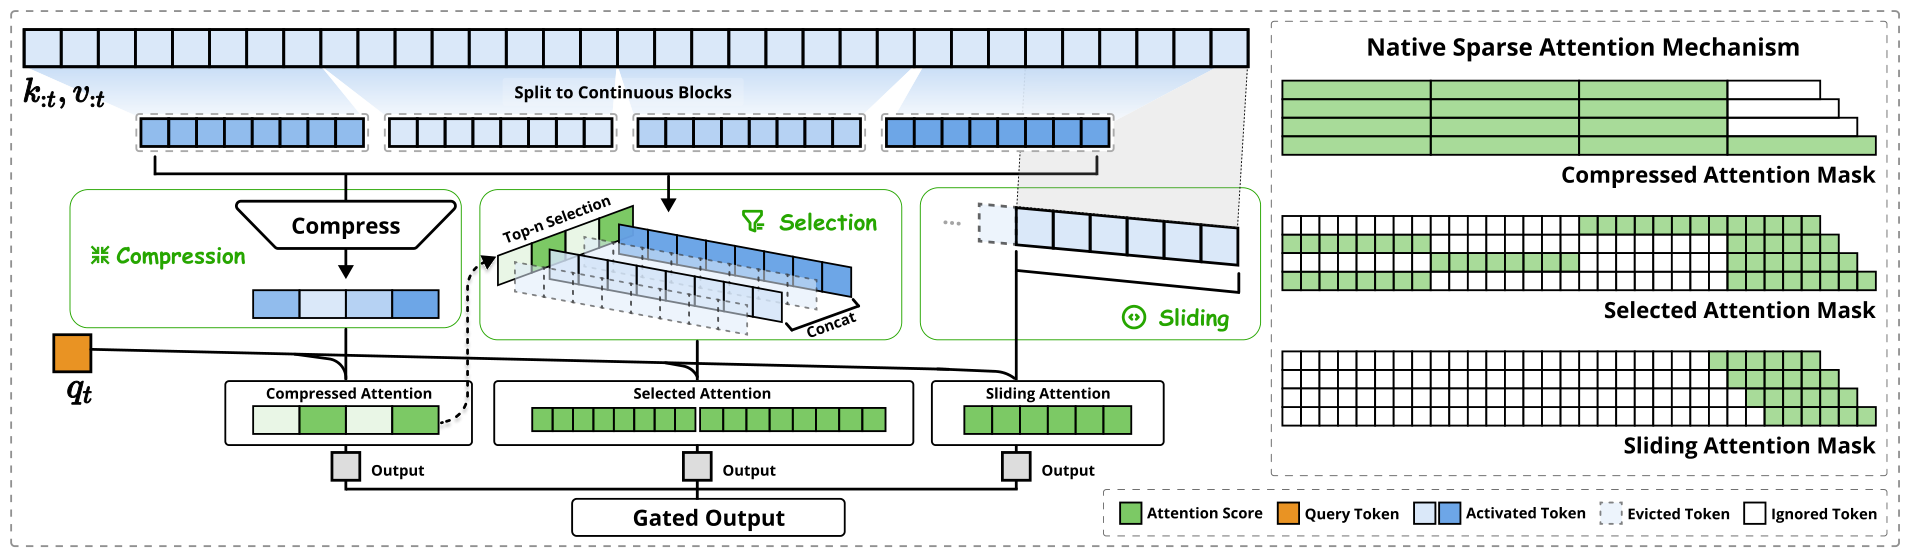
\includegraphics[width=\textwidth,height=0.33\textheight,keepaspectratio]{images/long-context/nsa_fig2_three_branches.png}\\[0.2em]
  {\scriptsize Left: the three branches; right: the masks they produce. Yuan et al., ``Native Sparse Attention: Hardware-Aligned and Natively Trainable Sparse Attention,'' ACL 2025, \href{https://aclanthology.org/2025.acl-long.1126/}{aclanthology.org/2025.acl-long.1126}, Figure~2.\par}
  \vspace{0.4em}
  \begin{columns}[T,onlytextwidth]
    \column{0.49\textwidth}
      \begin{itemize}\footnotesize\itemsep0.2em
        \item[\textcolor{red}{$\blacktriangleright$}] Yuan et al.\ (DeepSeek-AI, Peking University) give every query three branches, each with its own keys and values. In their 27B model:
          \begin{itemize}\scriptsize\itemsep0.1em
            \item \textbf{Compressed:} a small MLP maps each block of 32 keys (stride 16) to one coarse key.
            \item \textbf{Selected:} 16 blocks of 64 tokens at full resolution, always including the first block and the 2 most recent.
            \item \textbf{Sliding window:} the last $w = 512$ tokens, so fast-learned local patterns do not crowd out the other branches.
          \end{itemize}
      \end{itemize}
    \column{0.49\textwidth}
      \begin{itemize}\footnotesize\itemsep0.2em
        \item[\textcolor{red}{$\blacktriangleright$}] A learned gate mixes the branches:
          \[ o_t = \sum_{c\,\in\,\{\mathrm{cmp},\,\mathrm{slc},\,\mathrm{win}\}} g_t^{c}\, \mathrm{Attn}\big(q_t, \tilde K_t^{c}, \tilde V_t^{c}\big), \]
          where $\tilde K_t^{c}, \tilde V_t^{c}$ are the keys and values branch $c$ gives query $t$, and $g_t^{c} \in [0,1]$ is an MLP with a sigmoid on the token's features.
        \item[\textcolor{red}{$\blacktriangleright$}] Block scores come almost free: the compressed branch's probabilities $\mathrm{softmax}(q_t^{\top}\tilde K_t^{\mathrm{cmp}})$, summed over the heads of a GQA group.
      \end{itemize}
  \end{columns}
\end{frame}

\begin{frame}{NSA Is Trained Sparse From the Start}
  \begin{columns}[T,onlytextwidth]
    \column{0.50\textwidth}
      \begin{itemize}\footnotesize\itemsep0.3em
        \item[\textcolor{red}{$\blacktriangleright$}] \textbf{Kernel.} A kernel written in Triton, a Python-based GPU programming language, loads queries by GQA group. The group shares one block list, so each chosen block moves from HBM to SRAM once and serves every head in one dense matrix multiply.
        \item[\textcolor{red}{$\blacktriangleright$}] \textbf{Training.} No extra loss: the compressed branch that scores blocks is trained by the language-model loss through the gate.
        \item[\textcolor{red}{$\blacktriangleright$}] \textbf{Setup.} A 27B-parameter MoE (3B active) with GQA, pretrained on 270B tokens at 8k and adapted to 32k with YaRN, next to a full-attention twin.
        \item[\textcolor{red}{$\blacktriangleright$}] \textbf{Quality.} General benchmarks 0.456 against 0.443 (ahead on 7 of 9), LongBench long-document tasks 0.469 against 0.437, perfect needle retrieval at 64k.
        \item[\textcolor{red}{$\blacktriangleright$}] \textbf{Speed at 64k} on A100: forward 9.0$\times$ and backward 6.0$\times$ over Triton FlashAttention-2. A decoding step reads $n/16 + 16 \cdot 64 + 512 = 5{,}632$ tokens instead of 65,536, an expected 11.6$\times$.
      \end{itemize}
    \column{0.48\textwidth}
      \centering
      \vspace{0.8em}
      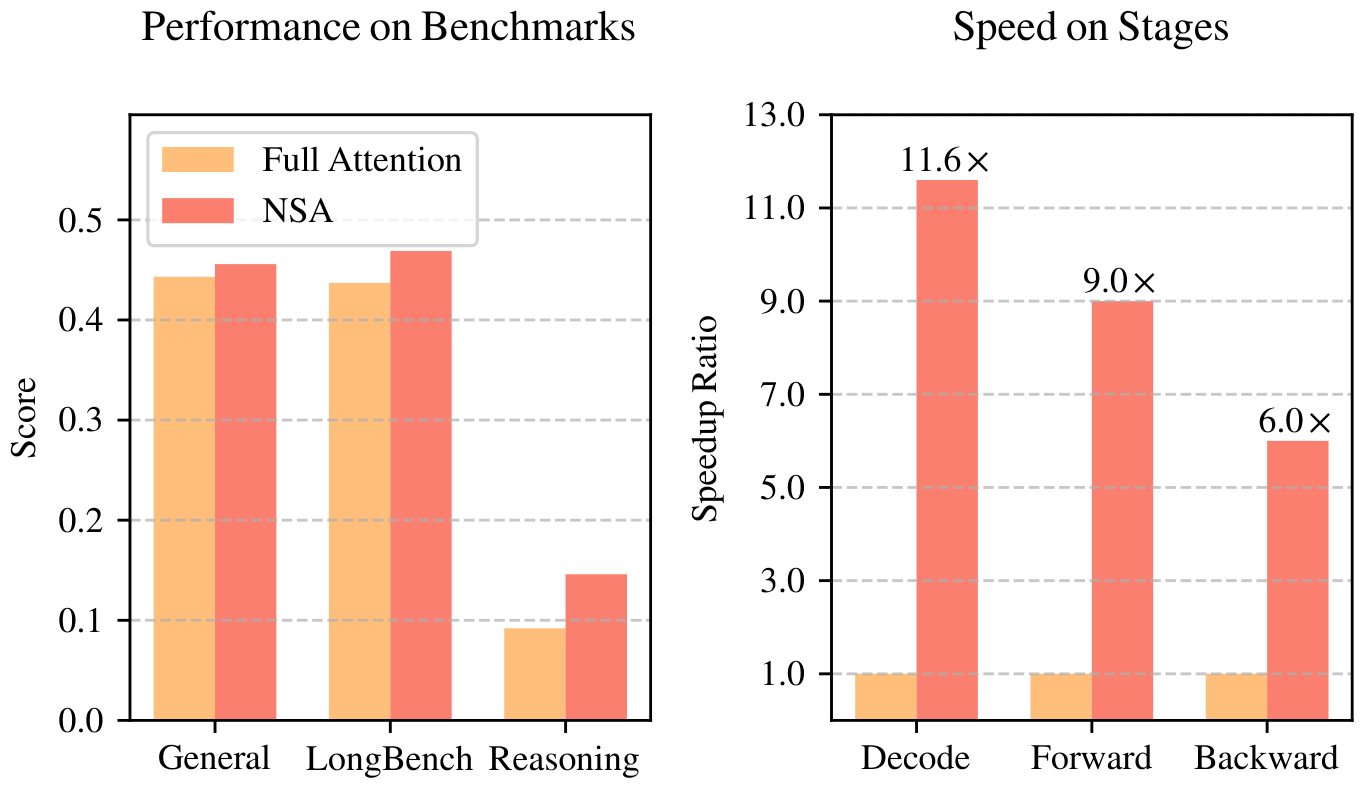
\includegraphics[width=\linewidth,height=0.50\textheight,keepaspectratio]{images/long-context/nsa_fig1_quality_and_speedup.png}\\[0.2em]
      {\scriptsize Left: average scores (``Reasoning'': AIME 2024 competition maths, after distillation); right: speedups at 64k. Yuan et al., \href{https://aclanthology.org/2025.acl-long.1126/}{aclanthology.org/2025.acl-long.1126}, Figure~1.\par}
  \end{columns}
\end{frame}

\begin{frame}{DeepSeek Sparse Attention: Token-Level Top-$k$}
  \begin{columns}[T,onlytextwidth]
    \column{0.50\textwidth}
      \begin{itemize}\footnotesize\itemsep0.3em
        \item[\textcolor{red}{$\blacktriangleright$}] DeepSeek-V3.2 has one architectural change from DeepSeek-V3.1-Terminus: DeepSeek Sparse Attention (DSA), added by continued training.
        \item[\textcolor{red}{$\blacktriangleright$}] A \textbf{lightning indexer} scores each earlier token $u$ for query token $t$:
          \[ I_{t,u} = \sum_{j=1}^{H^{I}} \alpha_{t,j}^{I}\, \mathrm{ReLU}\big(q_{t,j}^{I} \cdot k_{u}^{I}\big), \]
          with $H^{I}$ the small number of indexer heads, $q_{t,j}^{I}$ and the weight $\alpha_{t,j}^{I}$ from token $t$, and $k_u^{I}$ from token $u$. It can run in 8-bit floating point (FP8).
        \item[\textcolor{red}{$\blacktriangleright$}] Each query keeps its $k = 2048$ top-scoring tokens and runs MLA on them in multi-query form, so one entry serves all heads. Core attention drops from $O(n^2)$ to $O(nk)$; the indexer stays $O(n^2)$ but is far cheaper.
      \end{itemize}
    \column{0.48\textwidth}
      \centering
      \vspace{0.2em}
      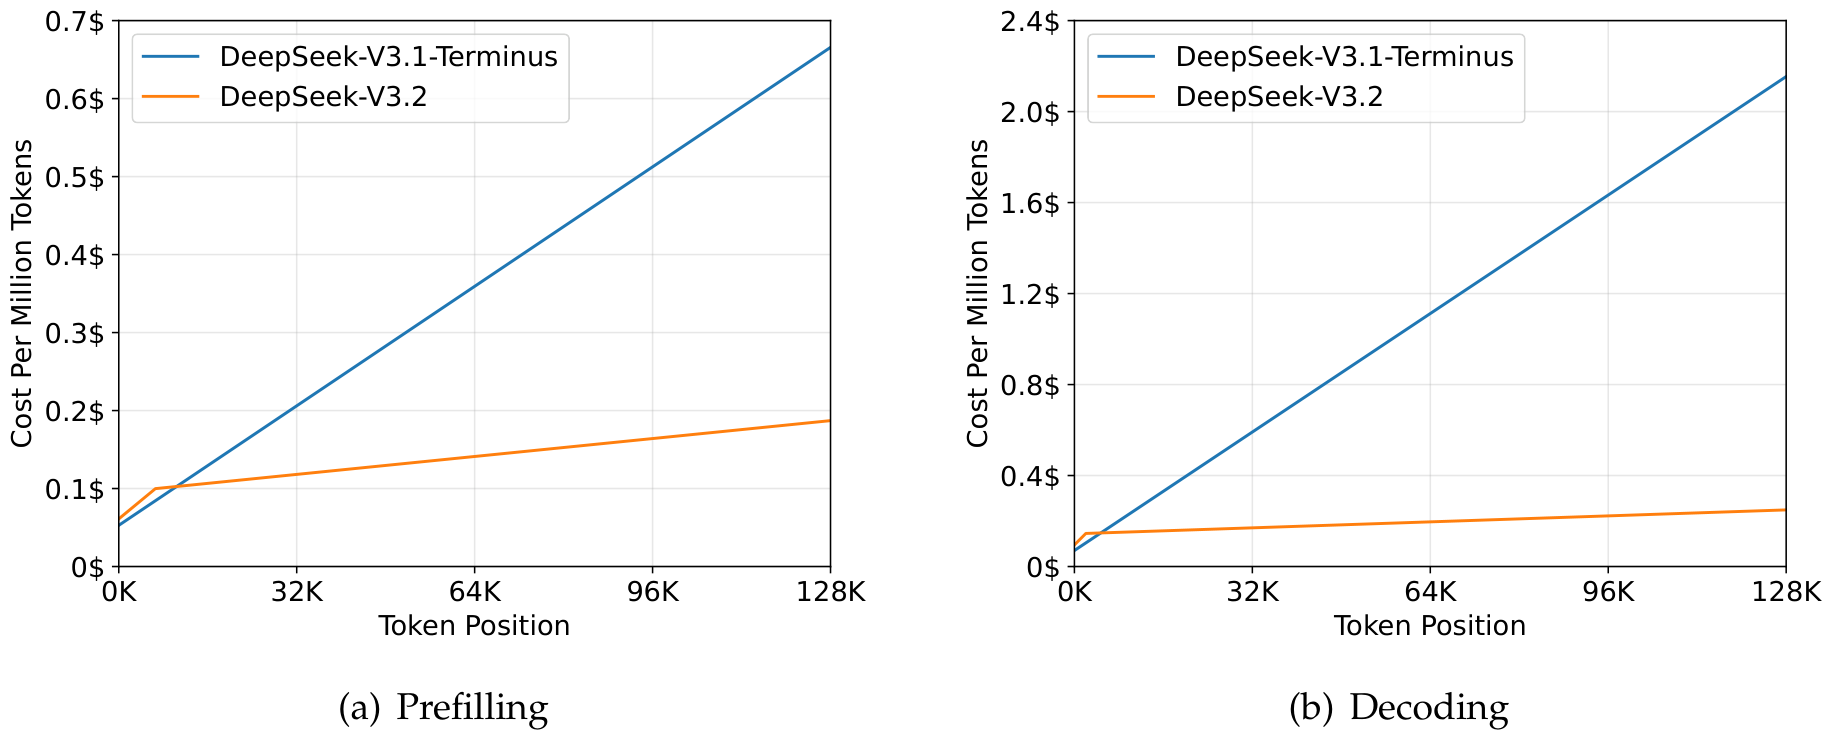
\includegraphics[width=\linewidth,height=0.40\textheight,keepaspectratio]{images/long-context/dsv32_fig3_inference_cost.png}\\[0.2em]
      {\scriptsize Cost per million tokens by position on H800 GPUs at 2 USD per GPU hour. At 128K, V3.1-Terminus against V3.2: \$0.67 vs \$0.19 (prefill), \$2.15 vs \$0.25 (decode). DeepSeek-AI, ``DeepSeek-V3.2: Pushing the Frontier of Open Large Language Models,'' 2025, \href{https://arxiv.org/abs/2512.02556v1}{arXiv:2512.02556v1}, Figure~3.\par}
      \vspace{0.3em}
      \begin{itemize}\footnotesize\itemsep0.2em
        \item[\textcolor{red}{$\blacktriangleright$}] \textbf{Warm-up:} attention stays dense; only the indexer trains, by a KL loss towards the head-summed attention. 1,000 steps, 2.1B tokens.
        \item[\textcolor{red}{$\blacktriangleright$}] \textbf{Sparse stage:} top-$k$ on, all weights train. 15,000 steps, 943.7B tokens of 128K sequences.
      \end{itemize}
  \end{columns}
\end{frame}

\begin{frame}{Four Ways to Choose Where to Look}
  \centering
  {\scriptsize
  \begin{tabular}{>{\raggedright\arraybackslash}p{1.35cm} >{\raggedright\arraybackslash}p{2.0cm} >{\raggedright\arraybackslash}p{2.7cm} >{\raggedright\arraybackslash}p{2.35cm} >{\raggedright\arraybackslash}p{3.1cm}}
    \toprule
    \textbf{Method} & \textbf{Unit selected} & \textbf{Selection signal} & \textbf{Sparsity added} & \textbf{What the kernel needs} \\
    \midrule
    Landmark (2023) & blocks (50 tokens in its language-model runs) & attention to one landmark token per block & pretraining or fine-tuning & block list per token and head; cache can sit in CPU memory \\
    \addlinespace[0.15em]
    MoBA (2025) & blocks of 256 to 4,096 & $q_t$ against mean-pooled keys; own block always kept & from scratch or continued; per-layer switch & queries regrouped by block, variable-length FlashAttention \\
    \addlinespace[0.15em]
    NSA (2025) & blocks of 64, coarse blocks, a window & compressed-branch attention, summed over a GQA group & from the first pretraining step & one block list per GQA group, contiguous loads into SRAM \\
    \addlinespace[0.15em]
    DSA (2025) & single tokens, $k = 2048$ & lightning indexer: a few ReLU heads in FP8 & continued: warm-up, then sparse stage & entries shared by all heads (multi-query MLA), not contiguous \\
    \bottomrule
  \end{tabular}\par}
  \vspace{0.6em}
  \begin{itemize}\footnotesize\itemsep0.3em
    \item[\textcolor{red}{$\blacktriangleright$}] All four cut compute and memory traffic per query, while the KV cache still grows with $n$ (Landmark can park it in CPU memory). The shared risk is a needed token outside the selected set; NSA's compressed branch and MoBA's dense last layers still see every position.
    \item[\textcolor{red}{$\blacktriangleright$}] Recurrent memory replaces the growing cache with a fixed-size state.
  \end{itemize}
\end{frame}
